\chapter{Background \& Objectives}

\section{Mammography}

Breast cancer is the leading cause of death among women and is the most common form of cancer found in women \cite{siegel2014cancer}. Early screening of breast cancer using mammography has been shown to reduce the mortality rate of women \cite{independent2012benefits, smith2014cancer}.

Mammography is the analysis of female breast tissue through the use of X-ray radiology with the goal of producing high resolution images of the structure within the female breast. The com- position of the parenchymal patterns and tissue density revealed by in a mammographic evaluation can be used in the early detection of breast cancer.

Qualitatively speaking the composition of breast tissue can be split into four distinct categories. These are Nodular densities (corresponding to Terminal Ductal Lobular Units (TDLUs), linear densities (corresponding to ducts, vessels, and fibrous strands), homogeneous, structureless densities (corresponding to fibrous supporting tissue), and radiolucent areas (corresponding to adipose tissue)\cite{tabar2005breast}. Typical markers used in the detection of cancer can are the presence of clusters of micro-calcifications, masses, architectural distortions, breast density and parenchymal patterns \cite{mccormack2006breast, sampat2005computer}.

There are two main projections used in X-ray mammography. These are known as craniocaudal (CC) and mediolateral oblique (MLO). Craniocaudal view is the "bottom-up" view of the breast and is the best method for visualising the medial aspect of breast tissue \cite{fischer2008breast}. The mediolateral oblique projection is a "side-on" view of the breast that provides maximum visualisation of the breast tissue in its entirety but is limited in its ability to visualise the inner breast tissue \cite{fischer2008breast}.

\subsection{Mammogram Acquisition}
The difference between high risk and low risk breasts is inherently small in mammogram due to the low level tissue contrast between the two classes \cite{kopans1998breast}. Because of this most essential part of mammographic imaging to ensure that a high contrast resolution is achieved in order to successfully capture the fine detail of the internal structures.

Mammopgraphic imaging has historically been carried using film but is now more commonly performed using digital mammography. Regardless of the medium the general technique for acquisition remains the same. The breast is placed on a plate between the X-ray tube and the detector. The breast is compressed from its normal conical shape onto the plate. This improves imaging by helping to ensure the X-ray attenuation through the breast tissue is as uniform as possible. 

Traditional film acquisition is hampered due to the film's sigmoid shaped response to x-ray exposure \cite{kopans1998breast}. This can lead to under or over exposure of the film which in turn leads to poor contrast. Digital mammography does not suffer from this issue because the response curve is essentially linear.


\subsection{Risk Assessment}
Mammograms provide a non-invasive means to assess the risk of a patient developing cancer. Several different systems have been developed to aid the classification of mammographic risk based on the parenchymal patterns visible through X-ray mammography.

\subsubsection{Wolfe}
The earliest attempt to classify mammographic risk using parenchymal patterns was suggested by Wolfe \cite{wolfe1976breast}. Wolfe proposed a classification system which split patients into four categories depending on the relative visible density of fat, ducts and connective tissue. The four categories are described, in order of lowest to highest risk, in ref. \cite{wolfe1976breast} as:

\begin{itemize}
	\item \textbf{N1} - Breast is mostly composed of fat with no visible ducts and very little amounts of dysplasia present. 
	\item \textbf{P1} - The parenchyma is primarily composed of fat with up to one quarter of the breast density being composed of visible ducts in the anterior position which may extend into a quadrant.
	\item \textbf{P2} - Breast indicates prominent duct pattern beyond one quarter of the breast that can occupy the entire parenchyma.
	\item \textbf{DY} - Breast is characterised by a severe increase in breast density and often appear as homogenous, missing the duct pattern present in P2 breasts.
\end{itemize}

\subsubsection{Boyd}
Boyd et al. \cite{boyd1995quantitative} proposed a quantitive assessment of risk based on increasing classes of mammographic density, known as the six class categories (SCC). These classes are based on the proportion of dense tissue relative to the area of the breast. The six classes are:

\begin{itemize}
	\item 0\%
	\item \textgreater 0 to \textless 10\% 
	\item 10 to \textless 25\% 
	\item 25 to \textless 50\%
	\item 50 to \textless 75\%
	\item $\geq$ 75\%
\end{itemize}

\subsubsection{Tab\'{a}r}
Tab\'{a}r et al. \cite{gram1997tabar} proposed a classification scheme which classifies a breast based on the percentage presence of the four building blocks of breast composition \cite{gram1997tabar, tabar2005breast}. The description of each of the five patterns is given as:

\begin{itemize}
	\item \textbf{Pattern I} - Breast corresponding to pattern I exhibit scalloped contours and cooper's ligaments with evenly scattered TDLU's.
	\item \textbf{Pattern II} - Complete fatty replacement of both
	\item \textbf{Pattern III} - Prominent retroareolar duct pattern and fatty involution.
	\item \textbf{Pattern IV} - Extensive linear and nodular densities present throughout the parenchyma.
	\item \textbf{Pattern V} - Homogeneous, structureless fibrosis with a convex contour.
\end{itemize}

\subsubsection{BI-RADS}
The Breast Imaging Report and Data System (BI-RADS) \cite{d1998illustrated, balleyguier2007birads} was developed by the American College of Radiology (ACR) in an attempt to standardise the lexicon used to describe mammography reports during standard screening. BI-RADS classifies the breast into four categories based on density \cite{balleyguier2007birads}.

\begin{enumerate}
	\item Fatty Breast (\textless10\% of dense tissue)
	\item Fibroglandular (10 - 49\% of dense tissue)
	\item Heterogeneously dense (49 - 90\% of dense tissue)
	\item Homogeneously dense (\textgreater 90\% of dense tissue)
\end{enumerate}

A radiologist will then classify the breast according to one of 7 categories after interpretation \cite{balleyguier2007birads}. These are one of:

\begin{itemize}
	\item Incomplete. Additional evaluation needed.
	\item Normal. 
	\item Typically benign.
	\item Probably benign. A shorter interval follow-up is recommended.
	\item Suspicious Abnormality. Biopsy considered.
	\item Highly suggestive of malignancy. Biopsy should be performed.
	\item Histologically proven malignancy.
\end{itemize}

\section{Features}
\label{sec:features}
Features are higher level descriptive abstractions computed from lower level structure such as areas of high intensity, edges, and corners present within an image. Features are the result of computing a descriptive property about an image from the intensity information contained within it. Hundreds of different types of features have been proposed \cite{cheng2006approaches, ganesan2013computer}. Broadly speaking, image features can be split into three distinct categories: shape (or morphological), intensity, and texture features. A brief review of some examples of each type are given in this section.

\subsection{Shape Features}
Shape features are features which detected within an image based on the morphological properties of a region of interest (ROI) within an image. The ROI could either be a suspicious artefact present in the mammogram, such as a malignant or benign tumour or cluster of micro-calcifications \cite{cheng2006approaches}, or it could simply be a property present in the parenchymal structure of the mammogram (which is the approach used in this project) such as regions of high density tissue \cite{chen2013multiscale} or prominent linear structures \cite{zwiggelaar1996finding}.

Typical example of features extracted from shapes of an ROI are the area covered by the shape, the circularity or rectangularity of the shape, and measures based on the perimeter of the shape \cite{petrick1999combined}. Additional features based on the normalised radial length (NRL) \cite{kilday1993classifying} such as boundary roughness, mean, entropy and area ratio \cite{petrick1999combined, petrick1996automated}, and statistics based on normalised chord length \cite{you1984performance} such as the first four statistical  moments of the resulting chord distribution \cite{el1996shape}.

\subsection{Intensity Features}
Intensity features are simple descriptive statistics based on the grey-level histogram of an image. Examples of such features are the mean, standard deviation/variance, skew, and kurtosis of the grey-level histogram of an ROI \cite{cheng2006approaches, christoyianni2000fast}.

\subsection{Texture Features}
Texture features are measurements of an image based on the repetition of patterns over an ROI \cite{parker2010algorithms}. Features based on the texture of an image are highly desirable because mammograms are obtained using a single medium of acquisition and the spatial distribution of features can be found in a single band \cite{ganesan2013computer}.

A set of commonly used set of texture features can be derived from the grey-level co-occurrence matrices (GLCM) \cite{haralick1973textural}. Grey-level co-occurrence matrices are used to describe the positions of pixels having similar grey-level values \cite{parker2010algorithms}. Pixel pairs within the GLCM are defined over a range of distances between pixels (often simply one) and orientations (often $0^\circ$ , $45^\circ$, $90^\circ$, and $135^\circ$). From GLCMs computed for each direction and orientation features representing texture context information such as  contrast, homogeneity, energy and entropy \cite{haralick1973textural, cheng2006approaches, parker2010algorithms} can be calculated.

Another approach to texture features uses the grey level difference statistics of a of an image vector. This takes the form of the absolute difference between pairs of grey levels within an image or between the average of local neighbourhoods. Like GLCM features, this technique is parameterised by the distances between the two image patches and the orientation of the distances used as an offset. First order statistics and measures of spread (such as entropy, contrast and angular second moment) can then the derived \cite{weszka1976comparative}.

One final approach to mammogram texture analysis is the use of a grey level run length statistics. This technique counts the number of consecutive occurrences of pixels with the same grey level value in a given orientation. Features are based on weighting longer or shorter runs as being more significant can then be created from the run length distribution \cite{weszka1976comparative, cheng2006approaches}.  

\section{Dimensionality Reduction}
Collections of features extracted from a set of images form a feature matrix (also known as as feature space) where each row in the matrix corresponds to a single image and each column corresponds to a single feature extracted from that image. Each entry in the matrix contains the value of a specific feature detected for that image. The number of columns in a feature matrix $m$ is known as the dimensionality of feature matrix. The goal of a feature matrix is that it encapsulates key information about what we are aiming to measure, allowing us to make inferences about what the data is telling us.

The field of dimensionality reduction is concerned with reducing the number of dimensions that a dataset has to only preserve the most important ones. In this way dimensionality reduction can be viewed as a feature selection method, discarding irrelevant or noisy dimensions in favour of those which best represent the data.

Dimensionality reduction techniques can be broadly split into two categories: linear and non-linear. As the name suggests linear approaches are restricted to representing data as a linear subspace while non-linear approaches are more versatile and can model more complex manifolds. 

Techniques used to perform dimensionality reduction can also be divided into those which are based on the principle or eigendecomposition (sometimes spectral decomposition)  \cite{strange2014open}. Methods with rely on this principle include Principle Component Analysis (PCA) \cite{shlens2014tutorial}, Isomap \cite{tenenbaum2000global}, and Locally Linear Embedding (LLE) \cite{roweis2000nonlinear} . Dimensionality reduction techniques which rely on eigendecomposition aim to factorise the feature matrix into the form:

\begin{equation}
	\bm{A} = \bm{Q}\bm{\Lambda}\bm{Q}^T
\end{equation}

Where $\bm{Q}$ is the the matrix of eigenvectors of $\bm{A}$ and $\bm{\Lambda}$ is a diagonal matrix containing the eigenvalues of $\bm{A}$. The lower dimensional representation of the feature matrix is then given by either the top or bottom eigenvectors in $\bm{Q}$.

Approaches not based on eigendecomposition include t-SNE and the SNE family \cite{van2008visualizing, hinton2002stochastic}, Autoencoder based approaches \cite{hinton2006reducing}, and Curvilinear Component Analysis \cite{demartines1997curvilinear}. SNE approaches focus on minimising the difference between probability distributions representing the higher and lower dimensional space. Autoencoders use a small number of middle nodes in a ANN to learn a compact representation of the data. Curvilinear component analysis builds on Sammon's mapping via minimisation of a cost function between distances in the representation but improves upon it by favouring local topology.

Another way of categorising dimensionality reduction techniques is whether they preserve local or global properties of the manifold. Since by definition of the problem a lower dimensional representation of a space cannot perfectly represent it there will always be a trade off in the accuracy of the mapping and number of discarded dimensions. Some approaches such as Isomap attempt to more accurately preserve the global properties of the data. Others such as t-SNE and LLE attempt to preserve the local neighbourhood structure at the expense of a less accurate representation of the global structure of the manifold.


\subsection{Curse of Dimensionality}
For some applications the dimensionality of a feature matrix may be quite small. Indeed it is trivial to ascertain the relationships between the features in a matrix where $m$ is equal to 2 or 3 by pure visualisation. However this is not the case when the feature matrix contains higher dimensional data where $m$ may be in the order of 100s or 1000s of features.

As the number of features (dimensionality) increases so does the volume of the feature space in which the data points are contained. This causes issues with any technique the requires statistical significance because a fixed number of data points will indefinitely become sparsely distributed as the dimensionality of the space increases. This is known as the curse of dimensionality \cite{bellman1965dynamic}.

This causes havoc with algorithms (such as classifiers) that depend on distance metrics such as Euclidean distance. The effect is such that in a very high dimensional space the distance pairs of data points becomes negligible in computations such as the nearest neighbour algorithm. All data points are effectively equally far away so the choice essentially become one of randomness \cite{domingos2012few}. 

However, often it is not the case that all of dimensions of a feature space are required in order to obtain a meaningful representation. Quite often the the data points in a feature space correspond to a lower dimensional manifold that is embedded within the higher dimensional feature space. Dimensionality reduction (also referred to as feature selection) techniques can be used to disregard noisy or irrelevant dimensions while still retaining meaningful information present in the higher dimensional space.

\subsection{Linear}
Linear approaches to dimensionality reduction make the assumption that the data in question lies approximately on a linear subspace within the higher dimensional representation. The core idea behind linear dimensionality reduction algorithms is to find the basis vectors representing the lower dimensional subspace.

\subsubsection{Principle Components Analysis}
Principle components analysis aims to preserve the maximal covariance of the data \cite{strange2014open}. First the covariance matrix of the feature space is computed via:

\begin{equation}
	C = \frac{1}{n}\Sigma \mathbf{x}_i \mathbf{x}_i^T
\end{equation}

Where $C$ is the co-variance matrix and $\mathbf{x}$ is the feature matrix. Eigendecomposition is then performed on the covariance matrix and to obtain the basis vectors for the subspace. Taking the first $n$ basis vectors creates a linear projection of the data onto a lower dimensional representation.

\subsection{Non Linear}
Often data points within the feature space do not lie on a linear subspace. Instead they are embedded in a non-linear manifold within a higher dimensional space. In this case taking a linear projection such as that produced by PCA will result in a distorted results with many parts of data overlapping with one another. However, linear techniques such as PCA are often useful as a preprocessing step to remove highly redundant or noisy dimensions before using a non-linear dimensionality reduction method.

\subsubsection{t-Distributed Stochastic Neighbour Embedding}
t-Distributed Stochastic Neighbour Embedding (t-SNE) \cite{van2008visualizing} is a non-linear dimensionality reduction technique which aims to preserve the distance between very similar data points. t-SNE models the high and low dimensional representations as joint probability distributions modelled using Student's t-distributions. The algorithm optimises the mapping by minimising the Kullback-Leibler divergence between the two distributions. In this way it models the probability that a higher dimensional point $p$ would choose $q$ as its neighbour. t-SNE can be used both with Euclidean distance or with other distance metrics.

\section{Quality Measures}
Performing dimensionality reduction on a dataset by definition causes a loss of information. The quality of the mapping produced by a dimensionality reduction algorithm can be measured by examining home the neighbourhood of a point in the higher dimensional data changes relative to the lower dimensional representation. In a good representation the neighbours in the higher dimensional space should be almost the same in the lower dimensional space. 

One way to quantify the quality of dimensionality reduction was suggested by Venna and Kaski \cite{kaski2003trustworthiness} is by measuring the trustworthiness and continuity of the mapping. If a mapping is trustworthy the $k$ closest neighbours in the original space will be neighbours in the projected space. Specifically the trustworthiness metric measures how many points in the low dimensional neighbourhood are not in the high dimensional neighbourhood. The trustworthiness measure is defined as:

\begin{equation}
	T = 1 - \frac{2}{Nk - 3k - 1} \sum\limits_{i=1}^N \sum\limits_{j \in U_k(i)} (r(i,j) - k)
\end{equation} 

Where $N$ is the number of samples, $r(i,j)$ is the rank of sample $j$ with respect to the distance from $i$ and $U_k(j)$ is the set of points that are in the neighbourhood of the low dimensional space but not the original space. The fraction $\frac{2}{Nk - 3k - 1}$ is used to scale the value to the range 0 to 1.

On the other side of the coin the quality of a mapping can be degraded by discontinuity. Discontinuity is effectively the reverse of the trustworthiness measure. If the neighbours exist in the neighbourhood of the original space but not in the mapping then the nature of the original space may not be preserved due to discontinuities in the projection. The measure of continuity is given by:

\begin{equation}
	C = 1 - \frac{2}{Nk - 3k - 1} \sum\limits_{i=1}^N \sum\limits_{j \in V_k(i)} (\hat{r}(i,j) - k)
\end{equation}

Where $N$ is the number of samples, $\hat{r}(i,j)$ is the rank of sample $j$ with respect to the distance from $i$ and $V_k$ is the set of points that are in the neighbourhood of the high dimensional space but not in the mapping. Again, the fraction $\frac{2}{Nk - 3k - 1}$ is use to scale the value to the range 0 to 1.

The measures of trustworthiness and continuity are closely related to the co-ranking matrix discussed by Lee and Verleysen \cite{lee2009quality}.

\section{Visualisation}
\label{sec:visualisation}
Traditionally plots of related low dimensional variables can be visualised directly using two or three dimensional scatterplots. However, direct visualisation of data with more than two or three dimensions is impossible with traditional methods. While dimensionality reduction techniques can be used to reduce the dimensionality of data down to two or three dimensions, it is unlikely that two or three dimensions are enough to accurately capture the structure of a complex higher dimensional manifold.

While a higher dimensional dataset cannot be directly visualised in the traditional sense, several different visualisation techniques have been developed that can be used to examine the structure present in higher dimensional data. This sections provides a brief review of several of these techniques.

\subsection{Scatterplot matrix}
A scatterplot matrices are possibly the simplest form of higher dimensional plot. Traditional scatterplots show the correlation between two variables. A scatterplot matrix is an $n \times n$ matrix of scatterplots where each individual plot shows the correlation between two variables i.e. the plot in row $i$ and column $j$ will show the plot of variables $X_i$ and $X_j$ 

\subsection{Parallel Coordinates}
Parallel coordinate plots \cite{inselberg1991parallel} show each variable as a single axis along the bottom of the graph. A single point on the plot is represented as a piecewise line across each of the axes. The position at which a point intersects an axis is the value of that the $n$-dimensional data point has for that variable.

There are some limitations to parallel coordinate plots. The principle limitation is that the effectiveness of the visualisation is dependant on the ordering of the axes. Different orderings will produce different visualisations. Sometimes the data naturally has a specific ordering (such as time-series data), however this is often not the case. Tatu et al. \cite{tatu2009combining} experimented with using the Hough transform to automatically infer "good" axis orderings. Johansson et al. \cite{johansson2009interactive} investigated ranking axis orderings using a combination of clustering, correlation and outlier features on the data. The scaling of each axis is also an important factor in the visualisation, however this can be solved by rescaling the data before visualisation.

\subsection{Andrews Plot}
An Andrews plot defines each $n$-dimensional data point as a Fourier series with $n$ terms. This visualisation is essentially the same as a parallel coordinates plot with each of the data points interpolated with Fourier interpolation. As such it suffers from the same limitations as parallel coordinates.

\subsection{RadViz}
RadViz \cite{novakova2009radviz} is a technique for visualising data points on a plane. RadViz models each $n$ dimensional data point as a single point on a 2D plane surrounded by a unit circle on which each of the $n$ features are placed equal distance apart from one another. Each data point is virtually ``connected" to each of the points on the unit circle via a ``spring". All of the springs are in equilibrium with one another and the final resting point for a point in the visualisation corresponds to the total strength exerted over point by each spring.

\section{Analysis}
This project aims to investigate the effect of mapping the feature space of both real and synthetic mammograms to a lower dimensional representation. This will involve the extraction of a variety of different shape, intensity, and texture features to produce a high dimensional feature space. We will then use dimensionality reduction techniques to produce a lower dimensional mapping and visualise the results using an appropriate technique. 

The hypothesis that we are aiming to test in the project is: Does the lower dimensional mappings of the higher dimensional feature space of synthetic mammograms match those of real patients? The high level questions that this project aims to answer are:

\begin{itemize}
	\item Are features which are important to real mammogram comparable to those of synthetic mammograms?
	\item If not, why are they different and does this relate to the author's own limitations?
	\item Can the knowledge gained be used to influence the perception of what features are important in a real mammogram?
	\item Could it be used to suggest how to build new mammogram models?
\end{itemize}

The technical work of the project will be concerned with implementing some existing approaches to feature extraction and dimensionality reduction in mammographic image analysis, but applying it to synthetic mammograms in order to evaluate the similarities and differences.

\begin{figure}
	\label{fig:pipeline-diagram}
	\centering
	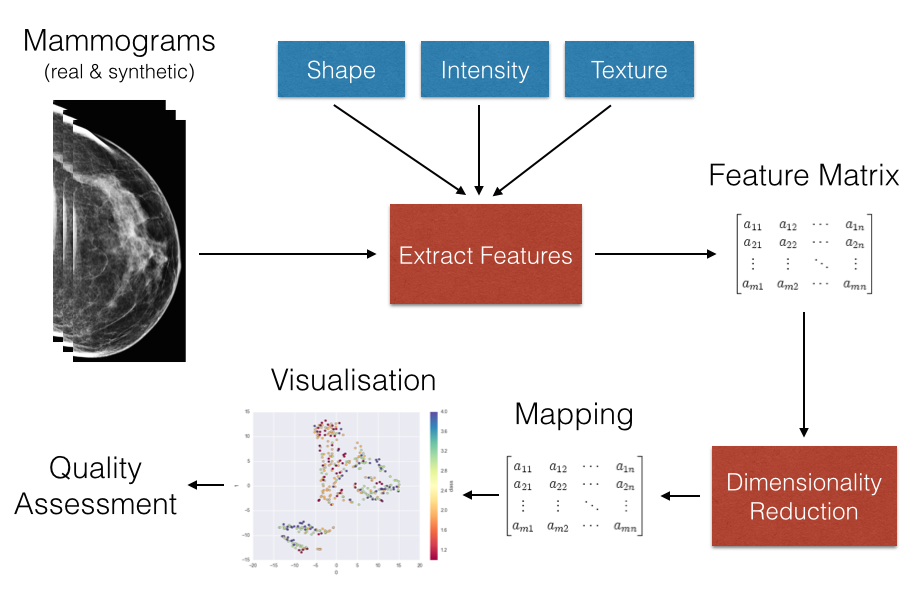
\includegraphics[width=0.8\textwidth]{Images/pipeline-diagram.png}	
	\caption{Conceptual overview of the image analysis pipeline to be produced as part of this project.}
\end{figure}

There are four core components of the methodology that need to be considered before implementation. The first is a decision on the number and type of features to be extracted from the images. Ideally the method used in this project should incorporate approaches that cover all three categories discussed in section \ref{sec:features}. This is so that a good variation in the discriminative properties of an image will be incorporated into the system. Focussing on only one technique for features considerably reduces the information that could be used to discriminate between images.

The second is the choice of dimensionality reduction techniques used to produce a lower dimensional mapping. Many different methods have been proposed for dimensionality reduction. It is highly likely relationship between variables in the feature space will not be a linear subspace. For this reason the chosen technique will almost certainly be a non-linear dimensionality reduction technique. However, it may be the case that the a linear dimensionality reduction technique such as PCA can be used to remove extremely redundant dimensions and reduce noise as a preprocessing step to a non-linear dimensionality reduction technique.    

Thirdly the lower dimensional mapping must be visualised. This may be done either directly if the mapping is to two or three dimensions. Alternatively the a higher dimensional plot such as those discussed in section \ref{sec:visualisation} could be used to higher examine the dimensional spaces. The choice of visualisation techniques will depend heavily on the choice of the two prior components. It is likely that the project will use a combination of different visualisation strategies depending on what specific aspect of the dataset is being examined. One of the issues with higher dimensional data is that it is impossible to produce visualisation that accurately capture all aspects of the data at once. Whatever technique is used will only ever show a projection of the feature space at best.

The final component of the system will be a form of quality measurement. While visual examination of the mapping is a necessity for qualitatively interpreting how the mapping is derived from the feature space, it is important to gain a quantitive measurement of the mapping. Quantitive measures can be used to check parameters for the dimensionality reduction algorithm are well configured and compare can compare between different combinations of features. 

\subsection{Choice of Language}
A technical decision must also be made regarding the choice of technologies and programming languages to be used as part of the project. All four components of the system are likely to be non-trivial to implement. Where possible existing implementations of parts of the four major components of this project should be used. The reasons for this are twofold. 1) using existing implementations should ensure that the development time is kept to a minimum, 2) they are likely to be better tested for validity. 

The programming language used as part of the system must be capable of easily implementing high level operations. It would be useful if the language of choice readily includes high level libraries for image processing and dimensionality reduction as well as statistical packages. At the time of writing there are several contenders for potential language choices to be used in this project. 

Python \cite{pythonLanguage} is one of the more obvious choices. The language community has several useful libraries for image processing such as scikit-image \cite{van2014scikit} and OpenCV bindings \cite{openCV} as well as dimensionality reduction such as scikit-learn \cite{pedregosa2011scikit}. It also has lots of general purpose high level libraries likely to be useful in this project such as NumPy \cite{pythonNumpy}, Scipy \cite{pythonSciPy} and Pandas \cite{pythonPandas}. For visualisation the matplotlib library seems like an obvious choice. An additional strength of python it is a very high level language that is perfect for rapid prototyping. The programmer does not need to concern themselves with the manual memory management or type system as in C, C++ or Java. However, this does not necessarily come with a loss in performance. Libraries such as Numpy and Scipy provide extremely quick pre-compiled high level operations written in C, allowing us to join performance with simplicity.

A strong alternative contender to Python is the R language \cite{rlanguage}. R was originally designed as a statistical programming language but has good support for many of the requirements of this project. Like python, R is a very high level scripting language which has many additional packages that can be installed such as packages for PCA \cite{rPCA}, t-SNE \cite{rtSNE}, LLE \cite{rLLE} etc. and the RIPA (R Image Processing and Analysis module) \cite{rRIPA}. For visualisation the excellent ggplot2 \cite{rggplot2} library is a clear candidate for this language.

Alternative languages which could be appropriate for this project include Matlab and C++. Like R and Python Matlab \cite{matlab} is a relatively high level language which has an extensive collection of libraries for data analysis and visualisation as well as support for image processing. However, the major downside to the Matlab application is that it is not free, even on a student license. The performance and object orientation offered by C++ are the major benefits offered and has direct support of the OpenCV library. However, as mentioned above the major downside C++ is the headaches of manual memory management and type system.s 

\section{Research Method}
The research method used in this project will be an experimental one. There will be an initial exploratory phase in which features, dimensionality reduction algorithms, visualisations and quality measures are tried and tested. Modifications will be made to existing approaches if necessary. Once an adequate implementation of both features, dimensionality reduction techniques, visualisation, and quality analysis has been achieved I will carry out the experiment with a subset of the real and synthetic mammogram datasets. I will use the largest possible subset from the real and synthetic datasets that I can as part of the experiment in order ensure the best possible representation of the feature space without over representing the subjects.

\section{Development Methodology}
The methodology for the implementation of the project will draw core on ideas from the agile development methodology. This software development methodology is the only one which makes sense for a research orientated project. Research orientated projects are by definition exploratory in nature and the results of the project cannot be stated in concrete at the start of the project. This rules out methodologies like waterfall and feature driven because in both systems the end result of development must be clearly stated up front, with little room for manoeuvre.

Agile approaches embrace change. This is a desirable attribute in a project where we can define the high level end goals of development but where the specifics must be flexible towards finding an approach that works based on analysis of the results from initial prototyping.

As this project is an individual endeavour the full power of an agile approach cannot be fully realised because some of the core principles rely interactions between multiple individuals (such as daily stand-up meetings and paired programming from XP).

There are however many other benefits to an agile approach that are relevant to an individual project. Test driven development (TDD) is a concept that is highly relevant. In software development TDD is used to ensure that you have confidence to make changes and verification that what you have written works. This is especially relevant and desirable in research projects because it not only gives you verification that the software is working, but can also be used to verify that the output of the program and therefore results are correct.

Short iterations and small releases that incrementally add value is another concept that is relevant to an individual project. This provides a measurable indicator of progress throughout the project. In this project I will aim to produce weekly iterations where I will select several stories to work on throughout the week. I will time the start of an iteration to coincide with the meeting with my postdoctoral supervisor who will effectively act as a ``customer" to the project. Work for the week will be decided based on discussions during these meetings so this naturally defines an anchor for iteration beginnings and endings.

Programmatic idioms associated with XP are also of value to an individual project. Simplicity (especially the concept of YAGNI) and heavy refactoring are likely to feature heavily in this project. Simplicity ensures that we keep the focus of the project limited to the goals of the research question without adding superfluous code that doesn't contribute to answering the questions outlined the problem analysis. Refactoring will allow the design of the project to be incremental. We can start with an initial basic design and rewrite and modify the structure of the code when it is needed in order to accommodate problems encountered or other change. In this way a good design (where verification of correctness is controlled by TDD) becomes a natural byproduct of development.


